
\begin{figure}[H]
  {
    \setlength{\tabcolsep}{3.0pt}
    \setlength\cmidrulewidth{\heavyrulewidth} % Make cmidrule = 
    \begin{adjustbox}{height=5cm,center}
      \footnotesize
      \begin{tabular}{ll}

        \makecell[l]{
\icode{.BYTE \$01,\$02}\\
\icode{.BYTE \$FF,\$FE}
} & \makecell[l]{

\includegraphics[width=1.3cm]{src/colorspace_patterns/pixels/pixel_pattern22_2.png}%

\includegraphics[width=1.3cm]{src/colorspace_patterns/pixels/pixel_pattern22_3.png}%
} \\
        \midrule

        \makecell[l]{
\icode{.BYTE \$01,\$00,\$FF}\\
\icode{.BYTE \$00,\$01,\$02}
} & \makecell[l]{

\includegraphics[width=1.3cm]{src/colorspace_patterns/pixels/pixel_pattern22_4.png}%
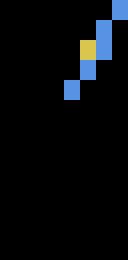
\includegraphics[width=1.3cm]{src/colorspace_patterns/pixels/pixel_pattern22_5.png}%
} \\
        \midrule

        \makecell[l]{
\icode{.BYTE \$00,\$FF,\$FE}\\
\icode{.BYTE \$02,\$03,\$04}
} & \makecell[l]{
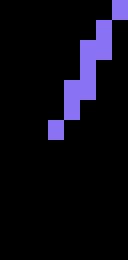
\includegraphics[width=1.3cm]{src/colorspace_patterns/pixels/pixel_pattern22_6.png}%
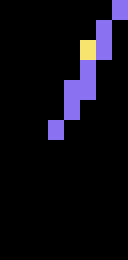
\includegraphics[width=1.3cm]{src/colorspace_patterns/pixels/pixel_pattern22_7.png}%
} \\
        \midrule

        \makecell[l]{
\icode{.BYTE \$FF,\$FE,\$FD}\\
\icode{.BYTE \$04,\$05,\$06}
} & \makecell[l]{

\includegraphics[width=1.3cm]{src/colorspace_patterns/pixels/pixel_pattern22_8.png}%
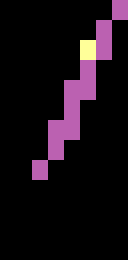
\includegraphics[width=1.3cm]{src/colorspace_patterns/pixels/pixel_pattern22_9.png}%
} \\
        \midrule

        \makecell[l]{
\icode{.BYTE \$FE,\$FD,\$FC}\\
\icode{.BYTE \$06,\$07,\$08}
} & \makecell[l]{
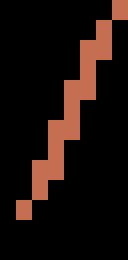
\includegraphics[width=1.3cm]{src/colorspace_patterns/pixels/pixel_pattern22_10.png}%
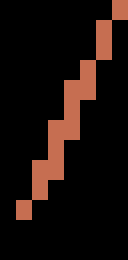
\includegraphics[width=1.3cm]{src/colorspace_patterns/pixels/pixel_pattern22_11.png}%
} \\
        \midrule

        \makecell[l]{
\icode{.BYTE \$FD,\$FC,\$FB}\\
\icode{.BYTE \$08,\$09,\$0A}
} & \makecell[l]{

\includegraphics[width=1.3cm]{src/colorspace_patterns/pixels/pixel_pattern22_12.png}%

\includegraphics[width=1.3cm]{src/colorspace_patterns/pixels/pixel_pattern22_13.png}%
} \\
        \midrule

          \end{tabular}
        \end{adjustbox}
      }\caption{Pattern Progression for 'User Lightform 12'}
    \end{figure}
    
